%NEURAL PRESY ;)

%----------------------------------------------------------------------------------------
%   PACKAGES AND THEMES
%----------------------------------------------------------------------------------------

\documentclass{beamer}

\mode<presentation> {

% The Beamer class comes with a number of default slide themes
% which change the colors and layouts of slides. Below this is a list
% of all the themes, uncomment each in turn to see what they look like.

%\usetheme{default}
%\usetheme{AnnArbor}
%\usetheme{Antibes}
%\usetheme{Bergen}
\usetheme{Berkeley}
%\usetheme{Berlin}
%\usetheme{Boadilla}
%\usetheme{CambridgeUS}
%\usetheme{Copenhagen}
%\usetheme{Darmstadt}
%\usetheme{Dresden}
%\usetheme{Frankfurt}
%\usetheme{Goettingen}
%\usetheme{Hannover}
%\usetheme{Ilmenau}
%\usetheme{JuanLesPins}
%\usetheme{Luebeck}
%\usetheme{Madrid}
%\usetheme{Malmoe}
%\usetheme{Marburg}
%\usetheme{Montpellier}
%\usetheme{PaloAlto}
%\usetheme{Pittsburgh}
%\usetheme{Rochester}
%\usetheme{Singapore}
%\usetheme{Szeged}
%\usetheme{Warsaw}

% As well as themes, the Beamer class has a number of color themes
% for any slide theme. Uncomment each of these in turn to see how it
% changes the colors of your current slide theme.

%\usecolortheme{albatross}
%\usecolortheme{beaver}
%\usecolortheme{beetle}
%\usecolortheme{crane}
%\usecolortheme{dolphin}
%\usecolortheme{dove}
%\usecolortheme{fly}
%\usecolortheme{lily}
%\usecolortheme{orchid}
%\usecolortheme{rose}
%\usecolortheme{seagull}
%\usecolortheme{seahorse}
%\usecolortheme{whale}
%\usecolortheme{wolverine}

%\setbeamertemplate{footline} % To remove the footer line in all slides uncomment this line
%\setbeamertemplate{footline}[page number] % To replace the footer line in all slides with a simple slide count uncomment this line

\setbeamertemplate{navigation symbols}{} % To remove the navigation symbols from the bottom of all slides uncomment this line
}

\usepackage{graphicx} % Allows including images
\graphicspath{ {images/} }
\usepackage{booktabs} % Allows the use of \toprule, \midrule and \bottomrule in tables
\usepackage{caption}
\usepackage{subcaption}
\usepackage{algorithm,algorithmic}
\usepackage{pgfplots}

\def\layersep{2cm}
\def\nodesep{0.25cm}
\usepackage{tikz, calc}
\newcommand*{\Scale}[2][4]{\scalebox{#1}{$#2$}}%
\newcommand*{\Resize}[2]{\resizebox{#1}{!}{$#2$}}%
\newcommand\sep{1.9cm}
\newcommand\height{0.9cm}
\usetikzlibrary{decorations.pathmorphing, backgrounds}
\tikzset{snake it/.style={decorate, decoration=snake}}
\usepgfplotslibrary{groupplots,units}

\usetikzlibrary{fit,intersections,}
%\usetikzlibrary{fit,intersections,}
\makeatletter
\tikzset{ % fitting node, see http://goo.gl/KOvpQ
  fitting node/.style={
    inner sep=0pt,
    fill=none,
    draw=none,
    reset transform,
    fit={(\pgf@pathminx,\pgf@pathminy) (\pgf@pathmaxx,\pgf@pathmaxy)}
  },
  reset transform/.code={\pgftransformreset}
}
\makeatother

%----------------------------------------------------------------------------------------
%   TITLE PAGE
%----------------------------------------------------------------------------------------

\title[General Artificial Neural Networks]{GANNs: A New Theory of Representation for \textbf{Nonlinear} Bounded Operators}
\author{William Guss}
\institute{Machine Learning at Berkeley}

%\author{William Guss}
\date{April 22, 2016} % Date, can be changed to a custom date
\makeatletter
\newcommand{\verbatimfont}[1]{\renewcommand{\verbatim@font}{\ttfamily#1}}
\makeatother
\begin{document}

\begin{frame}
\titlepage
\end{frame}

\section{Introduction}
\begin{frame}
\frametitle{Introduction: What's up with continuous data?} 
\begin{itemize}
	\item \textbf{All} of the data we deal with is discrete thanks to Turing.
	\item But, most of it models a continuous process.
	\item \textbf{Examples}
	\begin{itemize}
		\item Audio: We take $> 100k$ samples of something we could describe with $f: \mathbb{R} \to \mathbb{R}!$ 
		 Trick Question: Which is easier to use? (a) $v \in  \mathbb{R}^{100000}$ or (b) $f$.
		 \item Images: We take $100k\times 100k$ samples of something we could describe with $f:\mathbb{R}^2 \to \mathbb{R}$.
	\end{itemize}
	\item Why do we use discrete data? No computer known can really store $f.$ End of stoy.
\end{itemize}
\end{frame}

%------------------------------------------------

\begin{frame}
\Huge{\centerline{The End}}
\end{frame}


\begin{frame}
\Huge{\centerline{Jk}}
\end{frame}



\begin{frame}
\frametitle{Introduction: Abusing continuity}
\begin{itemize}
	\item $f$ can't be \emph{that} bad. Can it? 
	\item If $f$ is smooth it's easy to draw: \\
	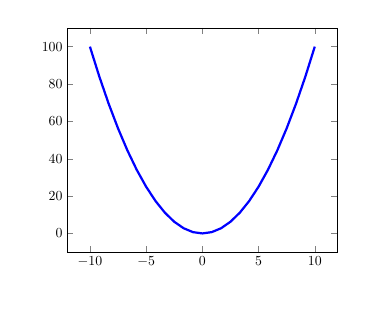
\begin{tikzpicture}[scale=0.5]
\begin{axis}
    \addplot[domain=-10:10, blue, ultra thick] {x^2};
\end{axis}
\end{tikzpicture}

\item I can even name $f$ most of the time: $f: x \mapsto x^2$ or even super precisely $ g: x \mapsto \sum_i^\infty a_n x^n $.
\item Moral: Smooth functions are mostly very managable.
\end{itemize}

\end{frame}


\begin{frame}

\frametitle{Introduction: Abusing continuity}
\begin{itemize}
	\item So why do we do this: \\
	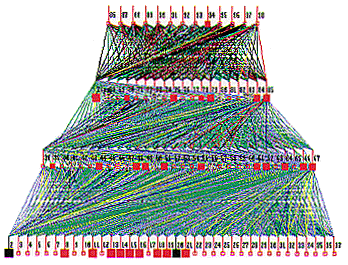
\includegraphics{sim2}
	\item To classify this:\\
	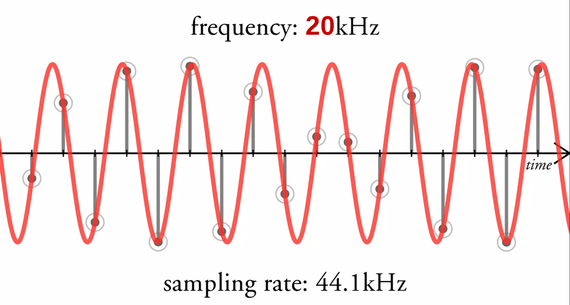
\includegraphics[width=0.5\textwidth]{20kHz-wave-Monty-Montgomery.png}
\end{itemize}

\end{frame}


\begin{frame}
\centering
\Huge{The Core Idea: Let neural networks abuse continuity and smoothness.}
\end{frame}

\section{The Core Idea}

\begin{frame}
\frametitle{Artificial Neural Networks}
From CS$189$-ish.
 \begin{definition}
    
    We say $\mathcal{N}: \mathbb{R}^n \to \mathbb{R}^m$ is a feed-forward neural network if for an input vector $\pmb{x}$,
    \begin{equation}
            \begin{aligned}
        \mathcal{N}:\ & \sigma_j^{(l+1)} = g\left(\sum_{i \in Z^{(l)}}w_{ij}^{(l)}\sigma_i^{(l)} + \beta^{(l)}\right) &\\  & \sigma_i^{(0)} \ \ \ =x_i& ,
        \end{aligned}
    \end{equation}
    where $1\leq l \leq L-1$. Furthermore we say $\{\mathcal{N}\}$ is the set of all neural networks.
    \end{definition}
\end{frame}


\begin{frame}
	\frametitle{Operator Neural Networks}
	Let's get rid of $\mathbb{R}^{100000}$ and use $f.$
	\begin{definition}
We call $\mathcal{O}: L^p(X) \to L^1(Y)$ an operator neural network if,
\begin{equation}
          \begin{alignedat}{2}
        \mathcal{O}:\ &\sigma^{(l+1)}(j) & &=  g\left(\int_{R^{(l)}} \sigma^{(l)}(i) w^{(l)}(i,j)\ di \right)  \\
        &\sigma^{(0)}(j) & &= f(j). 
        \end{alignedat}
\end{equation}
Furthermore let $\{\mathcal{O}\}$ denote the set of all functional neural networks.
\end{definition}
Well that was easy. In fact $\{\mathcal{O}\} \supset \{\mathcal{N}\}$ \\
\textbf{These definitions looks really similar? Is there some more general category or structure containing them.}
\end{frame}

\begin{frame}
	\frametitle{Generalized Artifical Neural Networks}
	 

	\begin{definition} If $A,B$ are (possibly distinct) Banach spaces over a field $\mathbb{F}$,
we say $\mathcal{G}: A \to B$ is a generalized neural network if and only if 

\begin{equation} \label{eq:gann}
          \begin{alignedat}{2}
        \mathcal{G}:\ &\sigma^{(l+1)} & &=  g\left(T_l\left[\sigma^{(l)}\right] + \beta^{(l)}\right)  \\
        &\sigma^{(0)} & &= \xi 
        \end{alignedat}
\end{equation}
for some input $\xi \in A$, and a linear form $T_l$.
\end{definition}
	\textbf{Claim:}
	"Neural networks" are powerful because they can move bumps anywhere! \\
	\emph{How?} $T_l$ is a linear form. It can move $\sigma^{(l)}$ anywhere, and $g$ is a bump of some sort.
\end{frame}

\begin{frame}
	\frametitle{Moving bumps around}
	\begin{itemize}
		\item The sigmoid function 
		\begin{equation}
			g = \frac{1}{1 + e^{-x}}
		\end{equation}
		is a bump, that we can move around with weights!
		\centering
		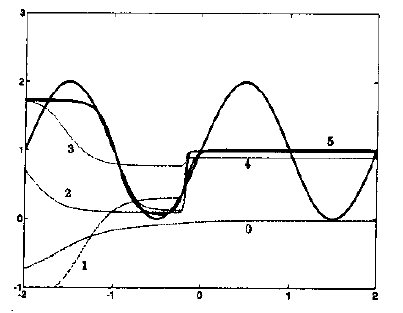
\includegraphics{20100524225320564.png}
	\end{itemize}
\end{frame}

\begin{frame}
	\frametitle{$T_l$ as the layer type.}
	\begin{definition}
We suggest several classes of $T_l$ as follows
  \begin{itemize}
  \item $T_l$ is said to be $\mathfrak{o}$ operational if and only if 
   =  \begin{equation} \label{eq:tlfunctional}
    \begin{aligned} 
      T_l = \mathfrak{o}: L^p(R^{(l)}) \to&\ L^1(R^{(l+1)}) \\
      \sigma \mapsto& \int_{R^{(l)}} \sigma(i) w^{(l)}(i,j)\ di.
    \end{aligned}
    \end{equation}
  \item $T_l$ is said to be $\mathfrak{n}$ discrete if and only if 
    \begin{equation} \label{eq:tldiscrete}
    \begin{aligned} 
      T_l = \mathfrak{n}: \mathbb{R}^n \to&\ \mathbb{R}^m \\
      \vec{\sigma} \mapsto& \sum_j^m \vec{e}_j\sum_i^n \sigma_i w^{(l)}_{ij}
    \end{aligned}
    \end{equation}
    where $\vec{e}_j$ denotes the $j^\mathrm{th}$ basis vector in $\mathbb{R}^m$.
  \end{itemize}
\end{definition}
\end{frame}

\begin{frame}
	\frametitle{$T_l$ as the layer type.}
	\begin{definition}
	\begin{itemize}
	  \item $T_l$ is said to be $\mathfrak{n}_1$ transitional if and only if 
    \begin{equation} \label{eq:tldiscrete}
    \begin{aligned} 
      T_l = \mathfrak{n}_1: \mathbb{R}^n \to&\  L^q(R^{(l+1)}) \\
      \vec{\sigma} \mapsto& \sum_i^n \sigma_i w^{(l)}_i(j).
    \end{aligned}
    \end{equation}
  \item $T_l$ is said to be $\mathfrak{n}_2$ transitional if and only if 
    \begin{equation} \label{eq:tldiscrete}
    \begin{aligned} 
      T_l = \mathfrak{n}_2: L^p(R^{(l)}) \to&\ \mathbb{R}^m \\
      \sigma(i) \mapsto& \sum_j^m \vec{e}_j\int_{R^{(l)}} \sigma(i) w^{(l)}_j(i)\ di
    \end{aligned}
    \end{equation}
	\end{itemize}
	\end{definition}
\end{frame}


\begin{frame}
	\frametitle{Neural networks as diagrams!}
	This generalization is nice from a creative standpoint. \\ 
	I can come up with new sorts of "classifiers" on the fly. \\

	\textbf{Examples:}
	\begin{itemize}
		\item A three layer neural network is just
		\begin{equation}
			\mathcal{N}_3: \mathbb{R}^{10000} \xrightarrow{g \circ \mathfrak{n}}\mathbb{R}^{30}  \xrightarrow{g \circ \mathfrak{n}} \mathbb{R}^{3}.
		\end{equation}
		\item A three layer operator network is simply
		\begin{equation}
			\mathcal{O}_3: L^p(R) 	 \xrightarrow{g \circ \mathfrak{o}} L^1(R) \xrightarrow{g \circ \mathfrak{o}} C(R).
		\end{equation}
		\item We can even classify functions!
		\begin{equation}
			\mathcal{C}:  L^p(R) 	 \xrightarrow{g \circ \mathfrak{o}} L^1(R) \xrightarrow{g \circ \mathfrak{o}} \dots \xrightarrow{g \circ \mathfrak{o}} L^1(R)\xrightarrow{g \circ \mathfrak{n}_2}  \mathbb{R}^n.
		\end{equation}
	\end{itemize}
\end{frame}

\section{Results}

\begin{frame}
	\frametitle{Results: Did abusing continuity help?}	 
	For every layer $\mathfrak{o}$ has weights
	\begin{equation}
		w^{(l)}(i,j) = 
    \sum_{b}^{Z^{(l)}_Y} \sum_{a}^{Z^{(l)}_X} k^{(l)}_{a,b}i^{a}j^{b}.
	\end{equation}


	\begin{theorem}
  Let $\mathcal{C}$ be a GANN with only one $\mathfrak{n}_2$ transitional layer with $O(1)$ weight polynomial. If a continuous function, say $f(t)$ is sampled uniformly from $t = 0$, to $t = N$, such that $x_n = f(n)$, and if $\mathcal{G}$ has an input function which is piecewise linear with  $O(N^2)$ weights.

  \begin{equation}
  \xi = \left(x_{n+1} - x_n\right)\left(z - n\right) + x_n
  \end{equation}

  for $n \leq z < n+1$, then there exist some discrete neural network $\mathcal{N}$ such that $\mathcal{G}(\xi) = \mathcal{N}(\pmb{x}).$
\end{theorem}
\end{frame}

\begin{frame}
	\frametitle{Results: Did abusing continuity help?}
	\textbf{WHAT!?!?} How did $\mathcal{C}$ reduce the number of weights from $O(N^2)$ to $O(1)?$
	\begin{itemize}
	 	\item The infinite dimensional versions of $\mathcal{N}$, in particular $\mathcal{O}$ and $\mathcal{C}$ are invariant to input quality. Takes the idea behind Convnets to an extreme!
	 	\item This is easy to see.
	 \end{itemize} 

	 	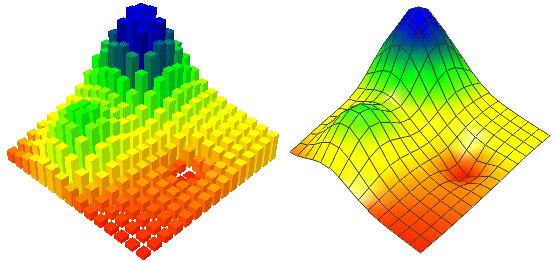
\includegraphics{gc082_1.png}
\end{frame}

\begin{frame}
	\frametitle{Results: Representation Theory}

	How good are Continuous Classifier Networks, $\{\mathcal{C}\}$ as algorithms? \\

	\begin{theorem}
		Let $X$ be a compact Hausdorf space. For every $\epsilon >0$ and every continuous bounded functional on $L^q(X)$, say $f$, there exists
		a two layer continuous classifier
		\begin{equation}
			\mathcal{C}: L^q(x) \xrightarrow{g \circ \mathfrak{n}_2} \mathbb{R}^m \xrightarrow{\mathfrak{n}} \mathbb{R}^n
		\end{equation}
		such that
		\begin{equation}
			\|f - \mathcal{C}\| < \epsilon.
		\end{equation}
	\end{theorem}

\end{frame}

\begin{frame}
	\frametitle{Results: Representation Theory}

	How good are Operator Networks and GANNs as algorithms? \\

	They should be able to approximate the important operators, eg. \textbf{Fourier Transform,} \textbf{Laplace Transform}, \textbf{Derivation}, etc.

\begin{theorem}
Given a operator neural network $\mathcal{O}$ then some layer $l \in \mathcal{O}$, the let $K:C(R^{(l)})\to C(R^{(l)})$ be a bounded linear operator. If we denote the operation of layer $l$ on layer $l-1$ as $\sigma^{(l+1)} = g\left(\Sigma_{l+1}\sigma^{(l)}\right)$, then for every $\epsilon >0$, there exists a weight polynomial $w^{(l)}(i,j)$ such that the supremum norm over $R^{(l)}$ \begin{equation}\left\|K\sigma^{(l)} -\Sigma_{l+1}\sigma^{(l)}\right\|_{\infty} < \epsilon\end{equation}

\end{theorem}
\begin{proof}
	See paper. Nice!
\end{proof}
\end{frame}

\begin{frame}
\frametitle{ICML}

\Huge{\centerline{Did you say bounded \textbf{linear?} }}	
\end{frame}

\begin{frame}
\frametitle{Results: Not as good as they sounded in my head.}
\begin{theorem}
Given a operator neural network $\mathcal{O}$ then some layer $l \in \mathcal{O}$, the let $K:C(R^{(l)})\to C(R^{(l)})$ be a bounded \textbf{linear} operator. If we denote the operation of layer $l$ on layer $l-1$ as $\sigma^{(l+1)} = g\left(\Sigma_{l+1}\sigma^{(l)}\right)$, then for every $\epsilon >0$, there exists a weight polynomial $w^{(l)}(i,j)$ such that the supremum norm over $R^{(l)}$ \begin{equation}\left\|K\sigma^{(l)} -\Sigma_{l+1}\sigma^{(l)}\right\|_{\infty} < \epsilon\end{equation}
\end{theorem}
\end{frame}

\begin{frame}
	\frametitle{Me}
	\centering
	
\includegraphics{stress.jpg}
\end{frame}


\begin{frame}
\frametitle{Results: Stronger Representation Theory }

We want to show the following better theorem.
\begin{theorem}
Given a operator neural network $\mathcal{O}$ then some layer $l \in \mathcal{O}$, the let $K:C(R^{(l)})\to C(R^{(l)})$ be a bounded \textbf{continuous} operator. If we denote the operation of layer $l$ on layer $l-1$ as $\sigma^{(l+1)} = g\left(\Sigma_{l+1}\sigma^{(l)}\right)$, then for every $\epsilon >0$, there exists a weight polynomial $w^{(l)}(i,j)$ such that the supremum norm over $R^{(l)}$ \begin{equation}\left\|K\sigma^{(l)} -\Sigma_{l+1}\sigma^{(l)}\right\|_{\infty} < \epsilon\end{equation}
\end{theorem}
But how? \textbf{Dirac Spikes!}
\end{frame}


\begin{frame}
\frametitle{Results: Stronger Representation Theory }

\only<1-4>{
\begin{tikzpicture}[scale=0.6]
	\begin{groupplot}[ 
	 group style = {group size=2 by 1, x descriptions at=edge bottom, vertical sep=0.2cm},
	axis lines=middle,
	width=9cm,
height=7cm,
  clip=true,
  ymin=-1,
  xticklabels=\empty,
  yticklabels=\empty,
  legend pos=north west]


  \nextgroupplot
	\addplot [mark=none, color=blue]{sin(deg(x))}; 
	\draw[fill=white] (axis cs:3.4,0.40) circle (0.0005) node[fitting node] (xi) {$\xi$} {};
	\draw[fill=white] (axis cs:3.4,0.70) circle (0.0005) node[fitting node] (xi) {$L^p(R)$} {};
         
	\nextgroupplot
	\addplot [mark=none, color=red]{x^2}; 

\draw[fill] (axis cs:4,16) circle [radius=1.5pt] node[above left] {\onslide<1-1>{$f$}\onslide<2->{$f(j)$} };
\draw[fill=white] (axis cs:4.5,20.5) circle [radius=1.5pt] node[above left] {\onslide<1-1>{$L^1(R)$}\onslide<2->{$\mathbb{R}$} };
\draw[fill] (axis cs:4,0) circle [radius=1.5pt] node[below right] {\onslide<1-1>{$\ $} \onslide<2->{$j$}};

\end{groupplot}
				\onslide<1-1>{ \draw[->] (7.5,4.8) -- (14,4.8) node [midway, above] {\tiny{$K, \mathcal{O}$}};}
            	\onslide<1-1>{\draw[|->] (6.6,3.9) -- (14,3.9) node [midway, above] {\tiny{$K, {?\above{\mathcal{O}}}$}}; }
            	\onslide<2->{\draw[|->] (6.6,3.9) -- (14,3.9) node [midway, above] {\tiny{$K_j, \mathcal{C}_j$}}; }
				\onslide<2-> {\draw[->] (7.5,4.8) -- (14.9,4.8) node [midway, above] {\tiny{$K_j, \mathcal{C}_j$}};}
\end{tikzpicture}
}
\only<5-7>{
	\begin{tikzpicture}[scale=0.6]
	\begin{groupplot}[ 
	 group style = {group size=2 by 1, x descriptions at=edge bottom, vertical sep=0.2cm},
	axis lines=middle,
	width=9cm,
height=7cm,
  clip=true,
  ymin=-1,
  xticklabels=\empty,
  yticklabels=\empty,
  legend pos=north west]


  \nextgroupplot
	\addplot [mark=none, color=blue]{0.5*sin(deg(x))};
	\addplot [mark=none, color=red!80]{0.7*cos(deg(x))};
	\addplot [mark=none, color=blue!70]{0.005*x^2 -0.003*x^3 +0.002*x^4};
	\addplot [mark=none, color=gren!100]{-x*0.4*cos(deg(x-0.5))};
	        \legend{$w_{1j}$, $w_{2j}$, $w_{3j}$, $w_{4j}$ } ;


	\nextgroupplot
\addplot3[surf] {(x<3.5&&x>3)*0.5*sin(deg(y)) + (x<2.5&&x>2)*0.7*cos(deg(y)) +(x<1&&x>0.5)*(0.005*y^2 -0.003*y^3 +0.002*y^4) + (x>4&&x<4.5)*(-y*0.4*cos(deg(y-0.5)))};
\end{groupplot}
\end{tikzpicture}
}

\only<8-12>{
	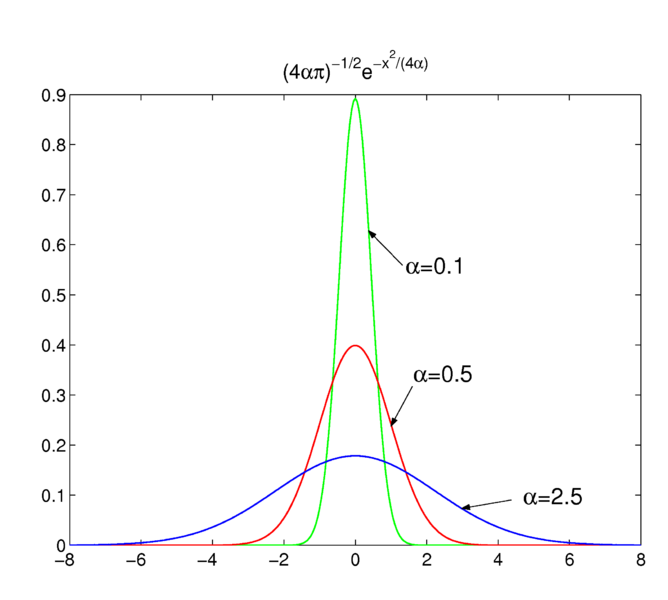
\includegraphics[width=0.4\textwidth]{Dirac_delta_gaussian.png}
	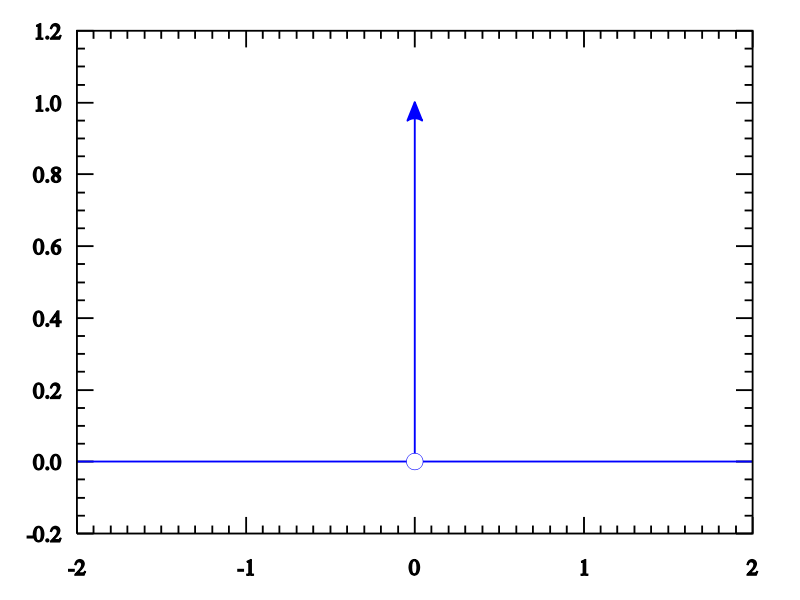
\includegraphics[width=0.4\textwidth]{Dirac_distribution_PDF.png}
}
\only<13->{
\centering
	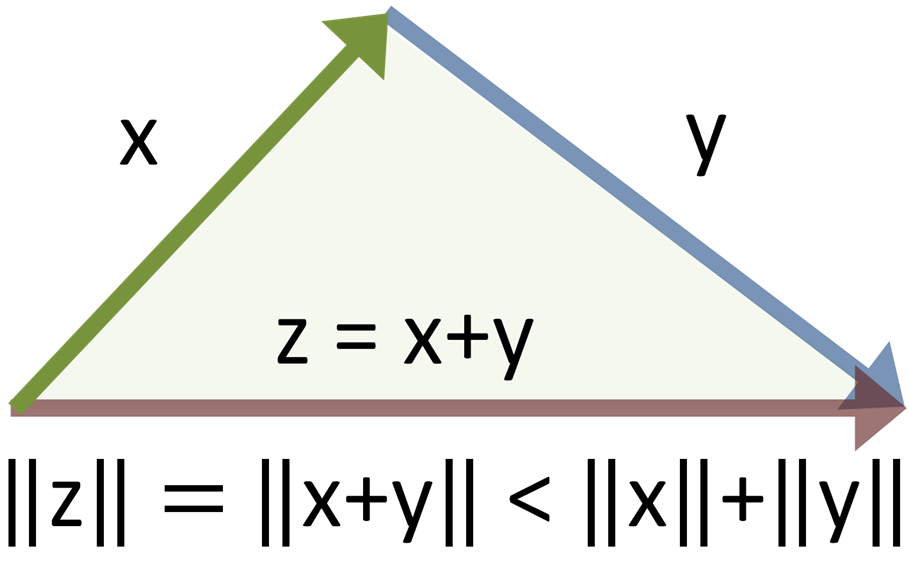
\includegraphics[width=0.5\textwidth]{Vector_triangle_inequality.PNG}
}

\begin{proof}
	\begin{itemize}
	 \only<2-3>{
		\item<2-3> Fix $\epsilon > 0$. Given $K: \xi \mapsto f$, let $K_j: \xi \mapsto f(j)$ be a functional on $L^q.$ 
		\item<3>  We can find a $\mathcal{C}_j:  L^q(R) \xrightarrow{g \circ \mathfrak{n}_2} \mathbb{R}^{m(j)} \xrightarrow{ \mathfrak{n}} \mathbb{R}^1$ so that for all $\xi$,
		\begin{equation}
			 |\mathcal{C}_j(\xi) - K_j(\xi)| = |\mathcal{C}_j(\xi) - f(j)| < \epsilon/2.
		\end{equation}
		}
		\only<4-4>{
			\item<4-4> We know that
			\begin{equation}
				\mathcal{C}_j(\xi) = \sum_{k=1}^{m(j)} a_{jk} g\left(\int_R \xi(i) w_{kj}(i)\ d\mu(i)\right)
			\end{equation}
		}
		\only<5-5>{
		\item<5-5> We wish to turn $C_j$ into a two layer $\mathcal{O}.$ Let, 
		\begin{equation*}
			w^{(0)}(i,\ell) = \left\{ 
				\begin{array}{lc}
					w_{kj}(i), & \text{if } $\ell = j+k$,  k\in{1,\dots,m(j)} 
					\\ 0 &\text{otherwise}
				\end{array}
				\right.
		\end{equation*}
		}
		\only<6-7>{
		\item<6-7> Then
		\begin{equation}
				\mathcal{C}_j(\xi) = \sum_{k=1}^m a_{jk} g\circ \mathfrak{o} [\xi](k+j) \right)
			\end{equation}
		\item<7-7> How do we turn this finite sum into an integral? Dirac time!
		}
		\only<8-8>{
		\item<8-8> We define a dirac spike as follows for every $n$:
		\begin{equation}
		 	\delta_{nkj}(\ell) = cn\exp(-bn^2{|\ell-(j +k)|^2})
		 \end{equation} 
		 where $c,b$ are set so that 
		 $\int_\mathbb{R} \delta_{nkj} = 1$
		}
		\only<9-9>{
		\item<9-9> Now let the second weight function be:
		\begin{equation}
			w_n^{(1)}(\ell,j) = \sum_{k=1}^m a_{jk}\delta_{nkj}(\ell)	
		\end{equation}
		}
		\only<10-10>{
		\item<10-10> Putting everything together, for every $n$ let $\mathcal{O}_n: L^p(R) \to L^1([0,1])$
		\begin{equation}
			\mathcal{O}_n : \xi \mapsto \int_{R} w^{(1)}(\ell, j) \mathfrak{o} [\xi](\ell)\ d\mu(\ell).
		\end{equation}
		Clearly $\mathcal{O}_n \to  \sum_{k=1}^m a_{jk} g\circ \mathfrak{o} [\xi](k+j) \right)$
		}
		\only<11-12>{
		\item<11-12> Therefore for every $\epsilon > 0$ there exists an $N$ such that for all $n > N$, for all $\xi$, and for all $j$,
		\begin{equation}
			|O_n[\xi](j) - C_j[\xi]| \leq \|\mathcal{O}_n[\cdot](j) - C_j[\cdot]\| < \epsilon/2.
		\end{equation}
		\item<12-12> Recall that for every $j$, $\|K_j - C_j\| < \epsilon/2.$
		}
		\only<13->{
		\item<13-> \textbf{TRIANGLE TIME!} By the triangle inequality we have that for all $j$
		\begin{equation}
			\begin{aligned}
				\|K_j - \mathcal{O}_n(k)\| = \|K_j -\mathcal{O}_n(j) + C_j -C_j\| \\
				 \leq \|K_j - C_j\| + \|\mathcal{O}_n(j) - C_k\| < \epsilon.
			\end{aligned}
		\end{equation}
		\item<14-> Therefore $\|K - \mathcal{O}\| < \epsilon $
		}
	\end{itemize}

\end{proof}
\end{frame}
%----------------------------------------------------------------------------------------

\begin{frame}
	\centering{\Huge{Phew that was a lot of math! Demo Time}}
\end{frame}

\end{document}
